\section{Double- and Single-Slit Experiments}
This document details the theory behind the single-slit and double-slit experiments as a way to describe how light interferes with itself as it passes through slits. In general, we will consider what happens when we shine light through a set of slits and look at the interference pattern on a screen a distance $D$ away, especially the distances $y$ from the center of the pattern to the locations of minimum/maximum intensity. 

\subsection{Double-Slit Experiment}
We already derived a similar version of this experiment for sound, but we will do it again (and also neglect the spherical nature of the wave).\\
Consider two infinitesimal slits a distance $d$ apart, and a light being shined through these slits. 
\begin{center}
	\begin{asy}
		import graph;
		size(200); 
real wall = 5; 
real D = 9;
real y = 4;
real d = 1.5;
pair sp1 = (0, d); 
pair sp2 = (0, -d); 
draw(Circle(sp1, 0.1)); 
draw(Circle(sp2, 0.1)); 
draw((D, -wall)--(D, wall)); 
draw((0, wall)--sp1+dir(90)*0.2, linetype("4 4")); 
draw((0, -wall)--sp2+dir(270)*0.2, linetype("4 4")); 
draw(sp2+dir(90)*0.2--sp1+dir(270)*0.2, linetype("4 4")); 
dot((D, y)); 
dot((0, 0)); 
draw((0,0)--(D, 0), linetype("4 4")); 
draw((0, -4)--(D, -4), Arrows);
dot((D, 0));
draw((D+0.5, 0)--(D+0.5, y), Arrows); 
draw((-0.5, d)--(-0.5, -d), Arrows);
draw(sp1+dir(25)*0.2--(D, y));
draw(sp2+dir(40)*0.2--(D, y));
draw((0, 0)--(D,y), linetype("8 8")); 

label("$d$", (-0.5, d)--(-0.5, -d), W);
label("$R$", (0,0)--(D,y), dir(140));
label("$y$", (D+0.5, 0)--(D+0.5, y), E);
label("$D$", (0+0.2, -4)--(D-0.2, -4), S);
label("$\theta$", (0,0), dir(12)*7);
	\end{asy}
\end{center}
For some chosen point a distance $y$ from the center, let $R$ be the distance from the midpoint of the slitss to this point, and $\theta$ to be the angle between the line to this point and the perpendicular to the center point. \\
We can compute the wave experienced at this point as the sum of two propagating waves (in exponential form): 
\[
	u(y, t) = \frac{1}{2} \left[ e^{i \left(k \sqrt{D^2 + \left(y - \frac{d}{2} \right)^2} - \omega t\right)} + e^{i \left(k \sqrt{D^2 + \left(y + \frac{d}{2} \right)^2} - \omega t\right)} \right]
\]
Note that taking the imaginary part of this expression will result in the sum of the waves we desire. Since we're mostly concerned where the maximum/minimum intensities are, we can use this exponential form of the wave to describe the wave. We also include the factor of $\frac{1}{2}$ to normalize the wave - it will scale the actual magnitude of the wave down by a factor of $2$, but it will not have an effect on which points will have a maximum/minimum intensity.\\
We will now make the approximation that $D >> d$, and use the Taylor series of the square root term, ignoring terms of second order or higher: 
\begin{align*}
	\sqrt{D^2 + \left(y - \frac{d}{2} \right)^2} &= \sqrt{D^2 + y^2 - yd + \left( \frac{d^2}{4} \right)} \\
	&= R \sqrt{1 - \frac{yd}{R^2} + \frac{d^2}{4R^2}} \\
	&= R \left[1 + \frac{1}{2}\left(\frac{d^2}{4R^2} - \frac{yd}{R^2}\right) - \frac{1}{8}\left(\frac{d^2}{4R^2} - \frac{yd}{R^2}\right)^2 + \ldots \right] \\
	&\approx R\left[1 - \frac{yd}{2R^2} \right] 
\end{align*}
We plug this approximation back into our original expression, using a similar approximation for the other square root: 
\begin{align*}
	u(y, t) &= \frac{1}{2} \left[ e^{i \left(kR - \frac{kyd}{2R} - \omega t\right)} + e^{i \left(k R + \frac{kyd}{2R} - \omega t\right)} \right] \\
	&= \frac{e^{i \left(kR - \omega t\right)}}{2} \left[ e^{- i\frac{kyd}{2R}} + e^{i\frac{kyd}{2R}} \right] \\
	&= e^{i \left(kR - \omega t\right)} \cos \left( \frac{kdy}{2R}\right) = e^{i \left(kR - \omega t\right)} \cos \left( \frac{kd}{2} \sin \theta \right)
\end{align*}
From this, we can see that we can maximize/minimize the amplitude, and thus, the intensity of the sound if we maximize/minimize the cosine term. \\
When the intensity of the sound is observed to be at a maximum, we should have that the argument of the cosine function should be $n \pi$ for some integer $n$ to have a maximum magnitude. This implies:
\[
	\frac{kd}{2}\sin \theta = n \pi  \rightarrow \frac{\pi d}{\lambda}\sin \theta = n \pi \rightarrow d\sin \theta = \lambda n 
\] 
Similarly, when the intensity of the sound is observed to be a minimum, the argument of the cosine function should be $\left( n + \frac{1}{2} \right) n$ for some integer $n$, so the magnitude of the intensity is minimized:
\[
	\frac{kd}{2}\sin \theta = \left( n + \frac{1}{2} \right) \pi  \rightarrow \frac{\pi d}{\lambda}\sin \theta = \left( n + \frac{1}{2} \right) \pi \rightarrow d\sin \theta = \lambda \left( n + \frac{1}{2} \right) 
\]
\subsection{Single-Slit Experiment and Diffraction Gratings}
What happens if the slits are no longer infinitesimal? Let's consider in this case shining light through a single slit of width $a$. By Huygens' Principle, every single point in the slit resembles a point source of light producing a spherical wave. In order to compute this, we consider $N$ infinitesimal slits with distance $d$ between each pair of slits, so $Nd = a$. To clarify our computation, we let $N$ be an odd positive integer (without loss of generality), and index each wave from $\frac{N-1}{2}$ to $-\frac{N-1}{2}$, where the wave indexed at $0$ emanates from the midpoint of the aperture. We also assume that the waves effectively behave as propagating waves rather than spherical waves to simplify calculations. 
\begin{center}
	\begin{asy}
		import graph; 
		size(200); 
		real wall = 5; 
		real D = 7;
		real y = 4;
		real a = 2.5;
		pair sp1 = (0, a); 
		pair sp2 = (0, -a); 
		draw(sp1+dir(180)*0.1--sp1+dir(0)*0.1); 
		draw(sp2+dir(180)*0.1--sp2+dir(0)*0.1); 
		draw((D, -wall)--(D, wall)); 
		draw((0, wall)--sp1); 
		draw((0, -wall)--sp2); 
		draw(sp2+dir(90)*0.2--sp1+dir(270)*0.2, linetype("4 4"));
		dot((0, 0)); 
		draw((0,0)--(D, 0), linetype("4 4")); 
		dot((D, 0)); 
		draw((D+0.5, 0)--(D+0.5, y), Arrows); 
		label("$y$", (D+0.5, 0)--(D+0.5, y), E);
		label("$D$", (0+0.2, -4)--(D-0.2, -4), S);
		dot((D, y)); 
        for (int i = -5; i < 6; ++i)	{
        	draw((D, y)--(0, a/6*i), linetype("2 2")+lightgrey);
        }
        //for (int i = 0; i < 6; ++i)	{
        	//draw(arc((0,0), 0.5+0.2*i, 60, -60));
        //}
		draw((0, -4)--(D, -4), Arrows);
		draw((0, 2)--(D,y), linetype("8 8")); 
		dot((0,2));
		label("$nd$", (-0.5, 2)--(-0.5,0), W);
		draw((-0.5, 2)--(-0.5,0), Arrows);
		draw((-1.5, a)--(-1.5, -a), Arrows);
		label("$a$", (-1.5, a)--(-1.5, -a), W);
		draw((0,0)--(D,y), linetype("8 8"));
		label("$\theta$", (0,0), dir(15)*7);
		label("$R$", (0,0)--(D,y), dir(320));
	\end{asy}
\end{center}
We can compute the waveform of the total wave experienced at a point $y$ from the center by summing up the exponential forms of each of the waves and considering the imaginary part to be our wave. We will normalize the overall wave with a factor of $\frac{1}{N}$. The wave experienced at a point $y$ is then: 
\[
	u(y, t) = \frac{1}{N} \sum_{n = -\frac{N-1}{2}}^{\frac{N-1}{2}} e^{i(k \sqrt{D^2 + (y - nd)^2} - \omega t)}
\]
We first look to simplify the square root. If we define $R = \sqrt{D^2 + y^2}$, and assuming $R >> d$, we can expand the square root using a Taylor series and eliminate second-order terms or higher: 
\begin{align*}
\sqrt{D^2 + (y - nd)^2} &= \sqrt{D^2 + y^2 - 2ndy + n^2d^2}\\
&= R \sqrt{1 - \frac{2ndy}{R^2} + \frac{n^2d^2}{R^2}} \\
&= R \left[1 + \frac{1}{2}\left(\frac{n^2d^2}{R^2} - \frac{2ndy}{R^2} \right) - \frac{1}{8}\left(\frac{n^2d^2}{R^2} - \frac{2ndy}{R^2}  \right)^2 + \ldots \right]\\
&\approx R \left[1 - \frac{ndy}{R^2} \right]
\end{align*}
We can substitute this back in and simplify, pulling out constants: 
\begin{align*}
u(y, t) &\approx \frac{1}{N} \sum_{n = -\frac{N-1}{2}}^{\frac{N-1}{2}} e^{i(kR\left[1 - \frac{ndy}{R^2} \right] - \omega t)} \\
&= \frac{e^{i(kR-\omega t)}}{N} \sum_{n = -\frac{N-1}{2}}^{\frac{N-1}{2}} e^{-i  \frac{kndy}{R}}
\end{align*}
This remaining sum is a geometric series, so we can evaluate it explicitly: 
\begin{align*}
u(y, t) &= \frac{e^{i(kR-\omega t)}}{N} \cdot \frac{e^{i \frac{kdy(N-1)}{2R}} - e^{i\frac{kdy(-N-1)}{2R}}}{1 - e^{-i\frac{kdy}{R}}} \\
&= \frac{e^{i(kR-\omega t)}}{N} \cdot \frac{e^{-i\frac{kdy}{2R}} \left(e^{i \frac{kdyN}{2R}} - e^{-i\frac{kdyN}{2R}} \right)}{e^{-i\frac{kdy}{2R}} \left(e^{i\frac{kdy}{2R}} - e^{-i\frac{kdy}{2R}} \right)} \\
&= \frac{e^{i(kR-\omega t)}}{N} \cdot \frac{2i \sin \left(\frac{kdyN}{2R} \right)}{2i \sin\left(\frac{kdy}{2R}\right)} \\
&= e^{i(kR-\omega t)} \cdot \frac{ \sin \left(\frac{kdyN}{2R} \right)}{N \sin \left(\frac{kdy}{2R}\right)} 
\end{align*}
In order to obtain a function for one slit, we can take the limit as $N \to  \infty$ and $d \to 0$ while holding $a$ constant. We can also take the liberty of substituting $\sin \theta = \frac{y}{R}$, as shown in the diagram:
\[
u(y, t) = \lim_{N \to \infty} e^{i(kR-\omega t)} \cdot \frac{ \sin \left(\frac{ka}{2} \sin \theta \right)}{N \sin \left(\frac{ka}{2N} \sin \theta \right)}
\]
Since $N \to \infty$, it is appropriate to use a small-angle approximation in the denominator and approximate $\sin \phi \approx \phi$ as the argument of the sine function approaches zero:
\[
 u(y, t) = \lim_{N \to \infty} e^{i(kR-\omega t)} \cdot \frac{ \sin \left(\frac{ka}{2} \sin \theta \right)}{N \cdot \frac{ka}{2N} \sin \theta}  \approx e^{i(kR-\omega t)} \cdot \frac{ \sin \left(\frac{ka}{2} \sin \theta \right)}{\frac{ka}{2} \sin \theta} 
\]
If we define $\sinc x = \frac{\sin x}{x}$, we have:
\[
	u(y, t) = e^{i(kR-\omega t)} \sinc \left(\frac{ka}{2} \sin \theta \right)
\]
We will only consider the points of minimum intensity in this waveform. Since intensity is proportional to the square of the amplitude, we have that the intensity will be minimized when $\sinc \left(\frac{ka}{2} \sin \theta \right) = 0$, and therefore:
\[
	\frac{ka}{2} \sin \theta = \pi n \rightarrow \frac{\pi a}{\lambda} \sin \theta = \pi n \rightarrow \frac{a \sin \theta}{n} = \lambda, n \in \ZZ
\]
Points of maximum intensity occur at the maxima of the $\sinc$ function, which are harder to compute (but still doable if we take a derivative, but there is no real nice form for these points). \\
It's worth noting that we can use a similar derivation for diffraction gratings with many slits. Consider our waveform for $N$ slits: 
\[
u(y, t) = e^{i(kR-\omega t)} \cdot \frac{ \sin \left(\frac{kdyN}{2R} \right)}{N \sin \left(\frac{kdy}{2R}\right)} 
\]
If we don't let $d \to 0$ and disregard the width of the grating $a$ while still letting $N \to \infty$, we get that the intensity of the waveform approaches zero in general (as the numerator is bounded between $-1$ and $1$ while $N$ is unbounded). The exception is when $\sin \left(\frac{kdy}{2R}\right)$ is close to zero (or equal to zero), where there exists a nontrivial intensity, since the reciprocal of a very small number is a very large number. This means maxima occur when: 
\[
\frac{kdy}{2R} = \frac{\pi d}{\lambda} \sin \theta = \pi n, n \in \ZZ \rightarrow d \sin \theta = n \lambda, n \in \ZZ
\]
From this, we see that the magnitude of the intensity of the wave, proportional to the amplitude squared, is proportional to the $\sinc$ function squared. The actual experimental single-slit diffraction pattern of a red laser is shown here: 
\begin{center}
	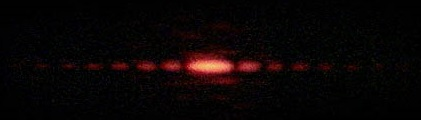
\includegraphics[scale=0.7]{images/waves/singleslitexp.jpg}\\
\end{center}
and the matching graph of the intensity distribution is here: 
\begin{center}
	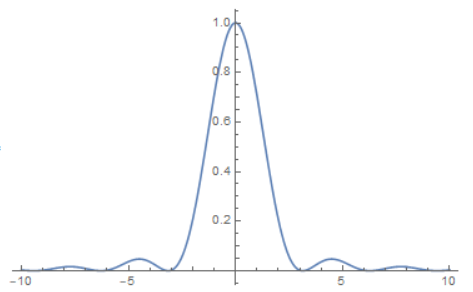
\includegraphics[scale=1]{images/waves/singleslitwaveform.png}\\
\end{center}
Notice the presence of a large central maximum and dimmer secondary maxima on either side of the center fading into darkness.
\subsection{Double-Slit Experiment Reloaded}
Of course, in reality, when we conduct the double-slit experiment, no matter how hard we pretend, the slits will have some width $a$, however small it may be. Suppose we now set up two slits of non-negligible width a distance $d$ apart and shine a light through these slits.\\
In order to derive the proper waveform for two slits of non-negligible width, we use a similar computation to the situation with a single slit, splitting up the width of the slit into infinitesimal slits and then taking an appropriate limit. Again, we invoke Huygens' Principle, so that every single point in each resembles a point source of light producing a spherical wave (except we neglect the spherical nature of the waves). Just as before, we consider $N$ infinitesimal slits with distance $\delta$ between consecutive infinitesimal slits, holding $N\delta = a$ constant, and assume that $N$ is an odd positive integer. We also use the same indexing scheme for each wave as in the single-slit derivation, letting $n$, a dummy variable, range from $-\frac{N-1}{2}$ to $\frac{N-1}{2}$ and indexing each infinitesimal slit from its distance from the center slit.  
\begin{center}
	\begin{asy}
		import graph; 
		size(200); 
		real wall = 5; 
		real D = 7;
		real y = 4;
		real a = 2.8;
        real d = 0.9; 
		pair s1L = (0, d); 
        pair s1U = (0, a+d);
		pair s2U = (0, -d); 
        pair s2L = (0, -a-d); 
		draw(s1L+dir(180)*0.1--s1L+dir(0)*0.1); 
		draw(s2U+dir(180)*0.1--s2U+dir(0)*0.1); 
        draw(s1U+dir(180)*0.1--s1U+dir(0)*0.1); 
		draw(s2L+dir(180)*0.1--s2L+dir(0)*0.1); 
        draw(s1L+0.1*dir(90)--s1U+0.1*dir(270), linetype("4 4")); 
        draw(s2L+0.1*dir(90)--s2U+0.1*dir(270), linetype("4 4")); 
		draw((D, -wall)--(D, wall)); 
		draw((0, wall)--s1U); 
		draw((0, -wall)--s2L); 
		draw(s2U--s1L);
		dot((0, 0)); 
		draw((0,0)--(D, 0), linetype("4 4")); 
		dot((D, 0)); 
		draw((D+0.5, 0)--(D+0.5, y), Arrows); 
		label("$y$", (D+0.5, 0)--(D+0.5, y), E);
		label("$D$", (0+0.2, -4)--(D-0.2, -4), S);
		dot((D, y)); 
        for (int i = -5; i < 6; ++i)	{
        	draw((D, y)--(0, d+a/2 + a/12*i), linetype("2 2")+lightgrey);
        }
        for (int i = -5; i < 6; ++i)	{
        	draw((D, y)--(0, -d-a/2 + a/12*i), linetype("2 2")+lightgrey);
        }
		draw((0, -4)--(D, -4), Arrows);
		draw((0, 0)--(D,y), linetype("8 8")); 
		draw((-0.5, d)--(-0.5, -d), Arrows);
		label("$d$", (-0.5, d)--(-0.5, -d), W);
        draw((-0.5, d)--(-0.5, a+d), Arrows);
		label("$a$", (-0.5, d)--(-0.5, a+d), W);
        dot((0,-3.2));
        dot((0,-2.3));
		label("$n\delta$", (-0.5, -2.3)--(-0.5, -3.2), W);
		draw((-0.5, -2.3)--(-0.5, -3.2), Arrows);
		draw((0, -3.2)--(D,y), linetype("8 8")); 
		label("$\theta$", (0,0), dir(15)*7);
		label("$R$", (0,0)--(D,y), dir(140));
	\end{asy}
\end{center}
From this setup, we have that the waveform $u(y, t)$ considering $2N$ infinitesimal slits is: 
\[
	u(y, t) = \frac{1}{2N} \left[\sum_{n = -\frac{N-1}{2}}^{\frac{N-1}{2}} e^{i \left(k \sqrt{D^2 + \left(y + \frac{a+d}{2} + n\delta \right)^2} - \omega t \right)} + \sum_{n = -\frac{N-1}{2}}^{\frac{N-1}{2}} e^{i \left(k \sqrt{D^2 + \left(y - \frac{a+d}{2} + n\delta \right)^2} - \omega t \right)} \right]
\]
Just as before, we will use a series of approximations and use a Taylor series expansion to expand the square roots. For simplicity, let's consider the first square root with all positive terms under the square root, as the second square root uses a similar procedure: 
\[
	\sqrt{D^2 + \left(y + \frac{a+d}{2} + n\delta \right)^2} = \sqrt{D^2 + y^2 + \frac{(a+d)^2}{4} + n^2 \delta^2 + 2yn\delta + y(a+d) + n\delta(a+d)}
\]
Just as before, we can factor out $R = \sqrt{D^2 + y^2}$:
\[
	= R\sqrt{1 + \frac{(a+d)^2}{4R^2} + \frac{n^2 \delta^2}{R^2} + \frac{2yn\delta}{R^2} + \frac{y(a+d)}{R^2} + \frac{n\delta(a+d)}{R^2}} \approx R \sqrt{1 + \frac{2yn\delta}{R^2} + \frac{y(a+d)}{R^2}}
\]
where the last step is the throwing out of negligible terms - these being $\frac{n^2 \delta^2}{R^2}$, $\frac{(a+d)^2}{4R^2}$, and $\frac{n\delta(a+d)}{R^2}$, as we assume $a, d, \delta << R$. We can now use the Taylor series expansion of $\sqrt{1+x}$, throwing out all terms after the first two non-zero terms: 
\[
	\approx R \left[1 + \frac{1}{2} \left( \frac{2yn\delta}{R^2} + \frac{y(a+d)}{R^2} \right) \right]
\]
Similarly, we can repeat the same process on the other square root and get: 
\[
	\sqrt{D^2 + \left(y - \frac{a+d}{2} + n\delta \right)^2} \approx R \left[1 + \frac{1}{2} \left( \frac{2yn\delta}{R^2} - \frac{y(a+d)}{R^2} \right) \right]
\]
We can plug back in and factor out the exponential terms that are common to both sums and independent of $n$: 
\begin{align*}
	u(y, t) &\approx \frac{1}{2N} \left[\sum_{n = -\frac{N-1}{2}}^{\frac{N-1}{2}} e^{i \left(k R \left[1 + \frac{1}{2} \left( \frac{2yn\delta}{R^2} + \frac{y(a+d)}{R^2} \right) \right] - \omega t \right)} + \sum_{n = -\frac{N-1}{2}}^{\frac{N-1}{2}} e^{i \left(k R \left[1 + \frac{1}{2} \left( \frac{2yn\delta}{R^2} - \frac{y(a+d)}{R^2} \right) \right]\right)} \right] \\
	&= e^{i(kR-\omega t)} \cdot \frac{1}{2N} \left[\sum_{n = -\frac{N-1}{2}}^{\frac{N-1}{2}} e^{i \left( \frac{kyn\delta}{R} + \frac{ky(a+d)}{2R} \right)} + \sum_{n = -\frac{N-1}{2}}^{\frac{N-1}{2}} e^{i \left( \frac{kyn\delta}{R} - \frac{ky(a+d)}{2R} \right)} \right] \\
	&= e^{i(kR-\omega t)} \cdot \frac{1}{2N}  \left( e^{i \frac{ky(a+d)}{2R}} + e^{-i \frac{ky(a+d)}{2R}} \right) \left[\sum_{n = -\frac{N-1}{2}}^{\frac{N-1}{2}} e^{i \frac{kyn\delta}{R}} \right] \\
	&= e^{i(kR-\omega t)} \cdot \cos\left( \frac{ky(a+d)}{2R} \right) \cdot \frac{1}{N} \left[\sum_{n = -\frac{N-1}{2}}^{\frac{N-1}{2}} e^{i \frac{kyn\delta}{R}} \right] 
\end{align*}
It now suffices to evaluate the remaining geometric series, simplifying as much as possible: 
\begin{align*}
	u(y, t) &= e^{i(kR-\omega t)} \cdot \cos\left( \frac{ky(a+d)}{2R} \right) \cdot \frac{e^{i\frac{ky\delta (1-N)}{2R}} - e^{i\frac{ky\delta (N+1)}{2R}}}{N \left( 1 - e^{i\frac{ky\delta }{R}} \right)} \\
	&= e^{i(kR-\omega t)} \cdot \cos\left( \frac{ky(a+d)}{2R} \right) \cdot \frac{e^{i \frac{ky\delta}{2R}} \left(e^{-i\frac{ky\delta N}{2R}} - e^{i\frac{ky\delta N}{2R}}\right)}{N e^{i\frac{ky\delta }{2R}} \left( e^{-i\frac{ky\delta }{2R}} - e^{i\frac{ky\delta }{2R}} \right)} \\
	&= e^{i(kR-\omega t)} \cdot \cos\left( \frac{ky(a+d)}{2R} \right) \cdot \frac{\sin \left( \frac{ky\delta N}{2R} \right)}{N \sin \left( \frac{ky\delta }{2R} \right)}
\end{align*}
Since $\delta << R$, we can use the small-angle approximation in the denominator $\sin x \approx x$ for sufficiently small values of $x$: 
\begin{align*}
	u(y, t) &\approx e^{i(kR-\omega t)} \cdot \cos\left( \frac{ky(a+d)}{2R} \right) \cdot \frac{\sin \left( \frac{ky\delta N}{2R} \right)}{ \frac{ky\delta N}{2R} } \\
	&= e^{i(kR-\omega t)} \cdot \cos\left( \frac{ky(a+d)}{2R} \right) \cdot \sinc \left( \frac{kya}{2R} \right)
\end{align*}
We can substitute $\frac{y}{R} = \sin \theta$, which gives:
\[
	u(y, t) = e^{i(kR-\omega t)} \cdot \cos\left( \frac{k(a+d)}{2} \sin \theta \right) \cdot \sinc \left( \frac{ka}{2} \sin \theta \right)
\]
Notice that the waveform is a product of the double-infinitesimal-slit waveform derived in the first section and the single-slit waveform derived in the section. This implies that the consideration of a non-negligible slit width simply superposes the single-slit distribution on top of the double-slit distribution. We can see this through an actual experiment: 
\begin{center}
	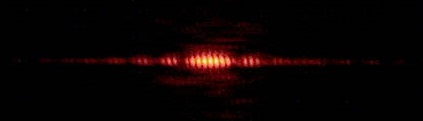
\includegraphics[scale=0.7]{images/waves/doubleslitexp.jpg}\\
\end{center}
or by means of graphing the intensity (which is proportional to amplitude squared): 
\begin{center}	
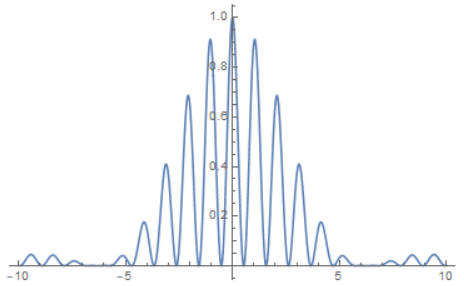
\includegraphics[scale=0.7]{images/waves/doubleslitwaveform.png}\\
\end{center}
As one can see from the graph and the experiment, the double-slit result is simply the result of the overlaying of the infinitesimal double-slit pattern (uniform, closely spaced peaks of intensity) and the single slit pattern (fading, large maxima out from the center). 